\chapter{}\label{ch:auf4}
Ab hier folgt der praktische Laborversuch.

\section{}\label{sec:4a}
\textit{Bestimmen Sie für diesen Motor mit Hilfe Ihrer Überlegungen aus der Aufgabe 3 die Polpaarzahl $ Z_{P} $.} \\
Wie wir in Abbildung \ref{fig:4a:flanken} erkennen können, befinden sich 2 fallende Flanken in einer Rotorumdrehung. Daraus können wir Schlussfolgern, dass die gesuchte Polpaarzahl des BLDC $ Z_{P} = 2  $ beträgt.
\begin{figure}
	\centering
	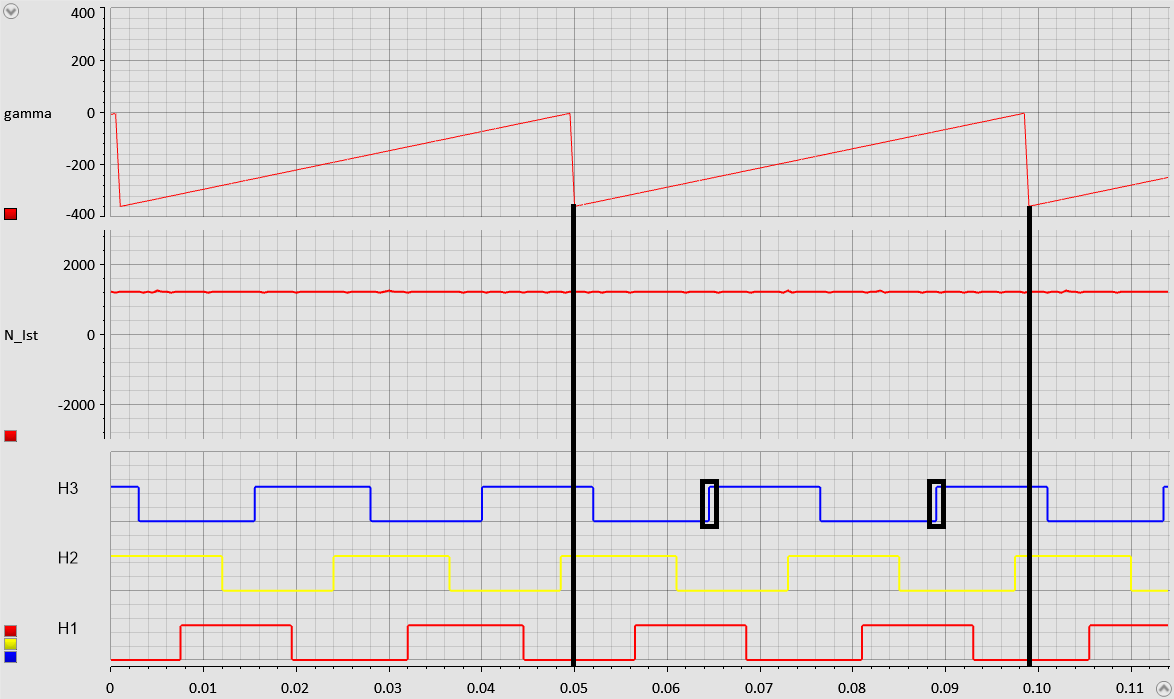
\includegraphics[width=0.99\textwidth]{./Bilder/BLDC_4a_markierung.png}
	\caption{Messung der Hallsensoren am Prüfstand}
	\label{fig:4a:flanken}
\end{figure}

\section{}\label{sec:4b}
\textit{Aufgabe ist es eine Ansteuerung für den Motor zu entwerfen, welche aus den gemessenen Hallsensorsignalen die Ansteuersignale für die Halbbrücken der Leistungselektronik liefert. Stellen Sie unter Verwendung Ihrer Überlegungen aus Aufgabe 2, eben jenen Zusammenhang in einer Tabelle dar.}\\
In Tabelle \ref{tab:4b:werte} sind die Ansteuersignale der Transistoren dargestellt. Wichtig hierbei zu wissen ist, dass sowohl im Zustand „000“, als auch im Zustand „111“, jegliche Transistoren gesperrt sind. Dadurch haben wir sichergestellt, dass dies jeweils sichere Zustände sind. Besonders zu beachten ist auch, dass keine zwei Transistoren eines Strangs gleichzeitig geschaltet werden, da sonst ein Kurzschluss stattfindet.\\
\begin{table}[h]
	\centering
	\begin{tabular}{p{1cm} p{1cm} p{1cm} | p{1cm} p{1cm} p{1cm} p{1cm} p{1cm} p{1cm}}
		&&&&&&&&\\[-1em]
		H1 & H2 & H3 & $ S_{UO} $ & $ S_{UU} $ & $ S_{VO} $ & $ S_{VU} $ & $ S_{WO} $ & $ S_{WU} $ \\
		\hline &&&&&&&&\\[-1em]
		  0 &  0 &  0 &   0 &   0 &   0 &   0 &   0 &   0 \\
		  0 &  0 &  1 &   0 &   0 &   1 &   0 &   0 &   1 \\
		  0 &  1 &  0 &   1 &   0 &   0 &   1 &   0 &   0 \\
		  0 &  1 &  1 &   1 &   0 &   0 &   0 &   0 &   1 \\
		  1 &  0 &  0 &   0 &   1 &   0 &   0 &   1 &   0 \\
		  1 &  0 &  1 &   0 &   1 &   1 &   0 &   0 &   0 \\
		  1 &  1 &  0 &   0 &   0 &   0 &   1 &   1 &   0 \\
		  1 &  1 &  1 &   0 &   0 &   0 &   0 &   0 &   0 \\
	\end{tabular}
	\caption{Wahrheitstabelle zur Ansteuerung der Transistoren}
	\label{tab:4b:werte}
\end{table}

\section{}\label{sec:4c}
Die Ansteuerung des BLDC für den Rechtslauf soll im Folgenden implementiert werden. Dafür haben wir die Schalttabelle erstellt, dem Programm die neuen Werte übergeben und dieses anschließend auf die Steuerung geladen.
